\chapter{Supplement to ``Community assembly on isolated islands:
  Macroecology meets evolution''}
\label{supp:ch2}

\section{Compilation of networks and metric validation}

Researchers have put forward a set of ``network metrics,'' including
nestedness \citep{bascompte2003, ulrich2009} and modularity
\citep{newman2004, olesen2007}, to understand the complex structure of
ecological networks. Null models are used to evaluate the statistical
significance of these metrics and to compare between networks of
different size \citep{ulrich2009}. We compare the results derived from
two common null models: the ``probabilistic null'' of
\cite{bascompte2003} using the relative degree distributions of plants
and herbivores as weights while randomizing links and suffers from
high Type II error \citep{ulrich2009}; the ``fixed-fixed null''
\citep{ulrich2009} maintains the exact number of links assigned to
each species while randomizing which interactors fill the requisite set
of links and suffers from high Type I error \citep{ulrich2009}. We find that
using these different null models does not change any trends in our
network statistics across the Hawaiian chronosequence but different
null models do influence the sign and significance of the network
metrics (Fig. \ref{figSupp:netMetComp}). We therefore do not interpret
the sing or significance of the metrics but only their relative trends
across site age.

Because these networks are based on opportunistic data associated with
species descriptions, and not based on standardized ecological
surveys, we cannot interpret patterns in network metrics without
evaluating possible sampling biases \citep{nielsen2007, gibson2011,
  rivera2012}.  To do so we rarify networks by the number of Hemiptera
species included and, for each subsampled network, re-calculate
nestedness and modularity z-scores. This rarefaction procedure shows
that nestedness is very sensitive to network size
(Fig. \ref{figSupp:rfy}), a known property of nestedness
\citep{nielsen2007, gibson2011, rivera2012}. However the relative
nestedness z-scores across networks remain qualitatively similar to
those observed for the complete networks (Fig. \ref{figSupp:rfy}).
Modularity depends on network size in a more variable way
(Fig. \ref{figSupp:rfy}). Modularity is expected to decrease with
network size \citep{rivera2012} and so the marked increase in
modularity with network size on Haleakala is unexpected. However in
light of the large number of highly specialized taxa this pattern is
more reasonable---if most species only have within module links then
removing these species through subsampling will only reduce overall
modularity.  Thus this pattern speaks to the high level of
specialization on Haleakala, and to a lesser extent at Kokee which
also shows a slight increase in modularity with network size
(Fig. \ref{figSupp:rfy}).


\section{\texttt{R} Scripts for Maximum Entorpy Analysis and Monte
  Carlo Methods}
\label{sec:meteCode}

\subsection{Needed Functions}

\begin{verbatim}
require(distr)

## d, p and r functions for the maxent link distribution
## also a funciton to calculate the MLE and log likelihood

dmelink <- function(x, la) {
    exp(-la*(x-1)) - exp(-la*x)
}

pmelink <- function(x, la, lower.tail=TRUE) {
    if(length(x) > 1) {
        cp <- sapply(x, function(q) sum(dmelink(1:q, la)))
    } else {
        cp <- sum(dmelink(1:x, la))
    }
    
    if(lower.tail) {
        return(cp)
    } else {
        return(1 - cp)
    }
}

rmelink <- function(n, la, X0) {
    sample(X0, n, rep=TRUE, prob=dmelink(1:X0, la))
}


qmelink <- function(x, la) {
    fun <- DiscreteDistribution(1:3000, dmelink(1:3000, la))
    fun@q(x)
}

## likelihood functions (for simple cases maxent solution is equivilant 
## to maximum likelihood solution so we use MLE for computational ease)
melink.mle <- function(x) {
    log(1 + 1 / mean(x - 1))
}

melink.logLik <- function(x) {
    la <- melink.mle(x)
    
    length(x) * log(1 - exp(-la)) - la * sum(x - 1)
}


## function to make rank function (for plotting) of maxent link distrib
melink.rankFun <- function(x) {
    qmelink(seq(1-1/(length(x)+1), 1/(length(x)+1), 
                by=-1/(length(x)+1)), melink.mle(x))
}

## mean squared error function for maxent link distrib
melink.mse <- function(x) {
    mean((sort(x, TRUE) - melink.rankFun(x))^2)
}

## monte carlo method for calculating distribution of mse values 
## under model where maxent truely generated the link distribution
sim.melink.z <- function(x, X0, nsim=999) {
    la <- melink.mle(x)
    
    res <- replicate(nsim, {
        # browser()
        sim <- rmelink(length(x), la, X0)
        return(melink.mse(sim))
    })
    
    obs.mse <- melink.mse(x)
    
    return(list(obs=obs.mse, z=(obs.mse - mean(res)) / sd(res), sim=res))
}
\end{verbatim}

\subsection{Example Use}

\begin{verbatim}
## set a Lagrange multiplier value and simulate data
la <- 0.01

## fit the maxEnt model to simulated data
x <- rmelink(2000, la, 2000)

## evalute if fitted maxEnt model matches the data
melink.mle(x) # the MLE should be near 0.01
plot(sort(x, TRUE)) # the plotted data should look like the theory
lines(pmelink(1:200, melink.mle(x)), col='red')

## test that the logLike function is returning the correct value
melink.logLik(x) - sum(log(dmelink(x, melink.mle(x)))) < 1e-12

## test that the log likelihood simulation is working
sim.melink.z(x, 200) # should be a small z-value
sim.melink.z(rbinom(100, 200, 0.1), 200) # should be a large z-value
\end{verbatim}

\printbibliography

\clearpage

\section*{Supplemental Figures}

\begin{figure}[!hp]
  \centering
  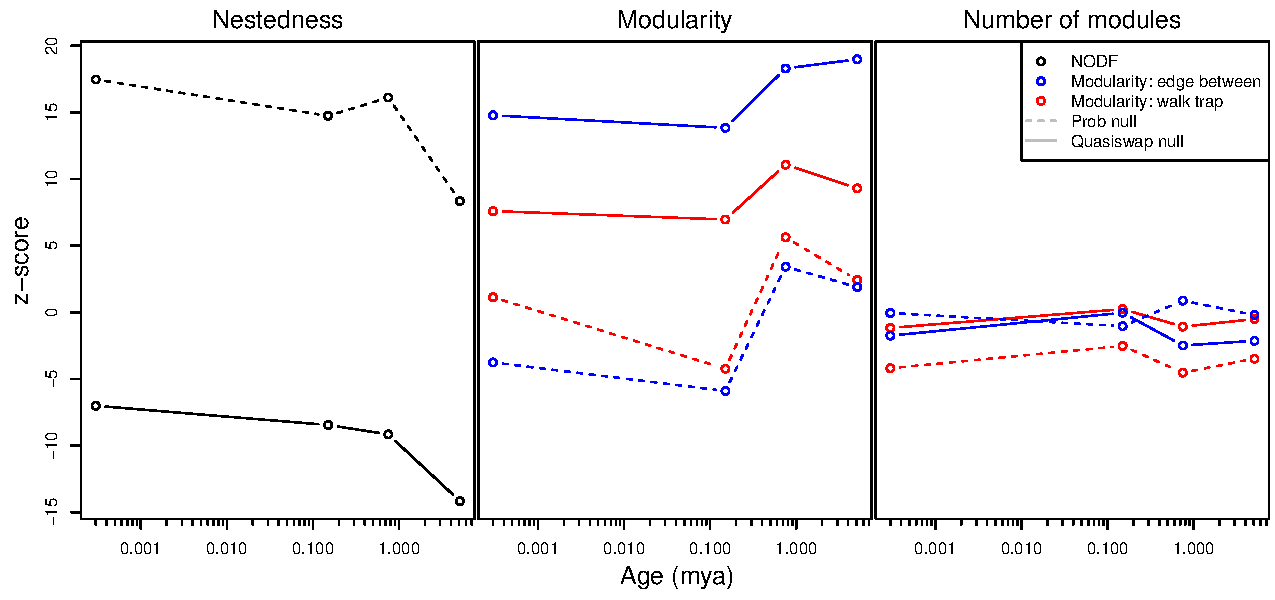
\includegraphics[scale=0.6]{figs/figSupp_netMetComp.pdf}
  \caption[Comparison of different null models]{Comparison of
    different null models (``Prob'' and ``Quasiswap'') used to
    standardize network metrics and comparison of different algorithms
    for assessing modularity (``edge between'' and ``walk
    drap''). Choice of null model has a strong influence on the sign
    and magnitude of metrics but not on their relative trends. The
    different modularity algorithms lead to largely similar
    qualitative patterns.}
  \label{figSupp:netMetComp}
\end{figure}

\begin{figure}[!hp]
  \centering
  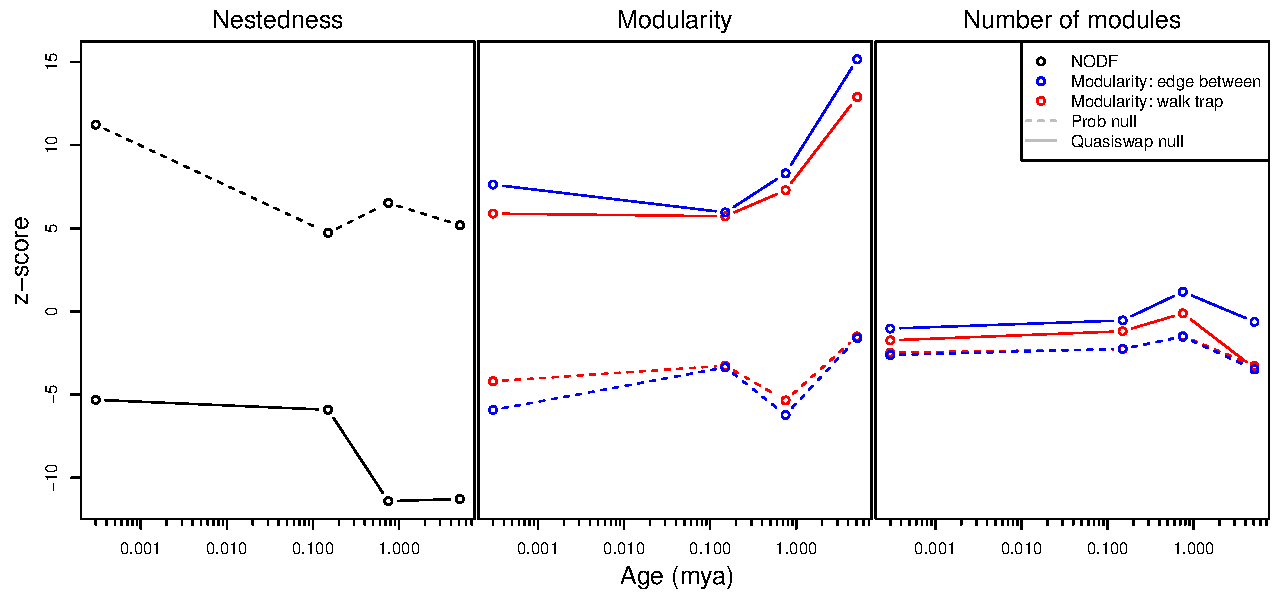
\includegraphics[scale=0.6]{figs/figSupp_netMetCons.pdf}
  \caption[NODF and modularity for non-conservative networks]{Metrics
    NODF and modularity calculated for networks based on more
    biogeographically conservative assignment of Hemiptera to
    localities. Colors and metric specifics as in Figure
    \ref{figSupp:netMetComp}.}
  \label{figSupp:netCons}
\end{figure}

\begin{figure}[!hp]
  \centering
  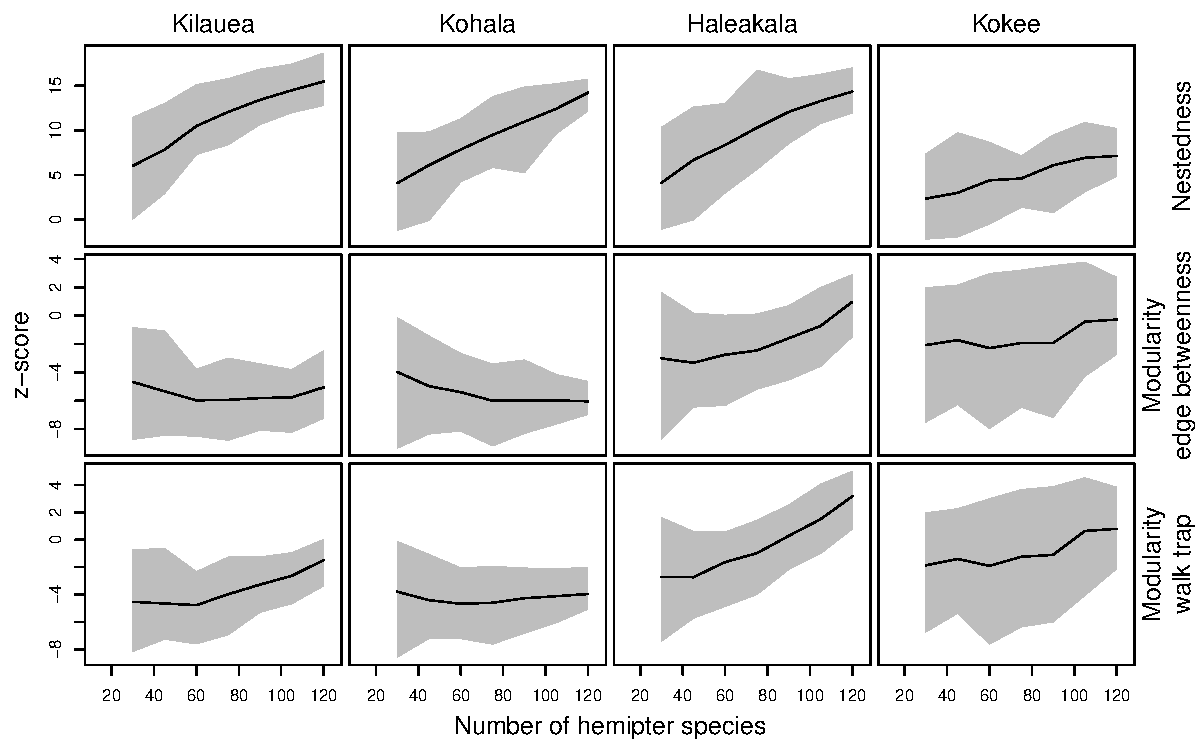
\includegraphics[scale=0.6]{figs/figSupp_rarified_prob1.pdf}
  \caption[Result from rarification analysis]{Result from rarification
    analysis showing sensitivity of network metrics to number of
    Hemiptera sampled.}
  \label{figSupp:rfy}
\end{figure}

